\documentclass[../Head/Main.tex]{subfiles}
\begin{document}
	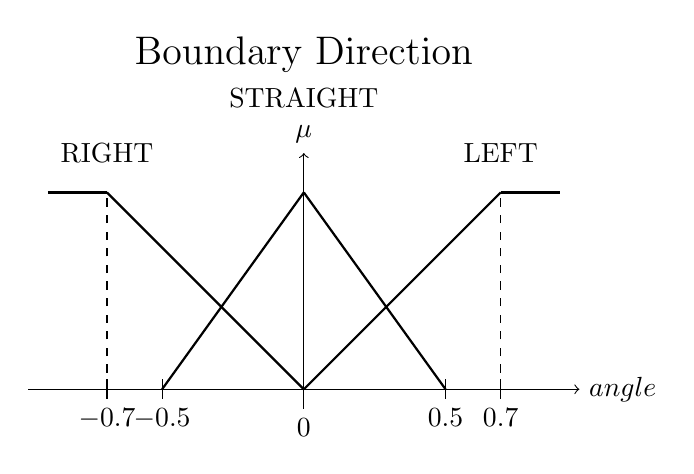
\begin{tikzpicture}
		\draw [->](3,-0.25)--(3,3) node[anchor = south]
			{$\mu$};
		\draw [->](-0.5,0)--(6.5,0) node[right]{$angle$};
		\node[anchor = north] at (3,-0.25) {$0$};
		
		\node at (3,4.25) {\Large Boundary Direction};
		\node at (0.5,3) {RIGHT};
		\node at (5.5,3) {LEFT};
		\node at (3,3.7) {STRAIGHT};	
		
		\draw (0.5,0.125) -- (0.5,-0.125) 
			node[anchor = north] {$-0.7$};
		\draw[dashed] (0.5,0) -- (0.5,2.5); 
			
		\draw (5.5,0.125) -- (5.5,-0.125)
			node[anchor = north] {$0.7$};
		\draw[dashed] (5.5,0) -- (5.5,2.5);
		
		\draw (1.2,0.125) -- (1.2,-0.125)
			node[anchor = north] {$-0.5$};
			
		\draw (4.8,0.125) -- (4.8,-0.125)
			node[anchor = north] {$0.5$};	
		
		\draw[thick] (-0.25,2.5) -- (0.5,2.5);
		\draw[thick] (5.5,2.5) -- (6.25,2.5);
		
		\draw[thick] (0.5,2.5) -- (3,0);
		\draw[thick] (5.5,2.5) -- (3,0);
		
		\draw[thick] (1.2,0) -- (3,2.5);
		\draw[thick] (4.8,0) -- (3,2.5);		
	\end{tikzpicture}
\end{document}